% Created 2016-03-30 Wed 06:58
\documentclass{article}
\usepackage[utf8]{inputenc}
\usepackage[T1]{fontenc}
\usepackage{fixltx2e}
\usepackage{graphicx}
\usepackage{longtable}
\usepackage{float}
\usepackage{wrapfig}
\usepackage{rotating}
\usepackage[normalem]{ulem}
\usepackage{amsmath}
\usepackage{textcomp}
\usepackage{marvosym}
\usepackage{wasysym}
\usepackage{amssymb}
\usepackage{hyperref}
\tolerance=1000
\usepackage{minted}
\usepackage{listingsutf8}
\usepackage[utf8]{inputenc} %% For unicode chars
\usepackage[bottom]{footmisc}
\usepackage[]{graphicx}
\usepackage{blindtext}
\usepackage[]{minted}
\usepackage[margin=1in]{geometry}
\usepackage{comment}
\usepackage[]{algorithm2e}
\usepackage[space]{grffile}
\setcounter{secnumdepth}{4}
\author{Nicholas Mitchell}
\date{\today}
\title{3\_Sentiment\_Analysis}
\hypersetup{
  pdfkeywords={},
  pdfsubject={},
  pdfcreator={Emacs 24.5.1 (Org mode 8.2.10)}}
\begin{document}

\maketitle
\tableofcontents


\section{Sentiment Analysis}
\label{sec-1}


\subsection{Sentiment analysis: definition and origins \label{sent-defn}}
\label{sec-1-1}
Also termed \emph{opinion mining}, \emph{sentiment analysis} describes a strategy that empowers machines to acquire subjective information, with the greater objective be the digitalisation of human emotion. It falls within the field of research known as \href{https://en.wikipedia.org/wiki/Natural_language_processing}{natural language processing (NLP)$^{\dag{}}$}, a term first appearing in the 1950's, as computers first began to receive more attention and people wondered whether they could be taught to learn - a classic example of the times being the Turing Test\footnote{Alan Turing introduced this idea in his paper: \href{https://en.wikipedia.org/wiki/Computing_Machinery_and_Intelligence}{Computing Machinery and Intelligence$^{\dag{}}$} \cite{turing1950computing}.} (Recent book covering it's history: \cite{Saygin2003}). NLP covers a broad spectrum of topics, and can best be summarised as the study of interaction between computers and humans, through the medium of their respective languages. On reporting significant progress in 1954 - successfully translating 60 sentences from Russian language to English language - researchers predicted (\cite{dostert1955georgetown}) that machine translation would be a solved problem within the decade. Over 60 years later and the problem persists, despite advances in linguistics and computing, and is likely to remain in this state for some time to come (see section \ref{SA-limits} for more on this).

The field of Sentiment Analysis is constantly evolving, enhancing existing models and creating new ones. This is, firstly, \emph{possible} due in part to new ideas and approaches towards NLP and also because of advancements in the technologies that are the engine behind such the analytical part, i.e. the algorithms. Secondly, the evolution is \emph{necessary} as to keep pace with the target subject. Natural languages are dynamic, changing over time, which makes a \emph{final solution} an unlikely outcome. A model defined today, which can perfectly quantify the sentiment of text (e.g. a tweet), offers little or no guarantee of performing so well next year. New words, expressions and configurations of the two are created on a daily basis, in all natural languages.

\vspace{5mm}
A thorough treatment of the sentiment analysis, its history and development is provided by Liu (2012) \cite{Liu:sentiment-analysis}. As the inclusion of \emph{sentiment} into financial models is somewhat of a divergence away from pure facts and statistics (at least in its essence), two further related books that explore this realm should be mentioned. The first is \href{http://irrationalexuberance.com/main.html?src\%3D\%252F}{\emph{Irrational Exuberance$^{\dag{}}$}} \cite{shiller2015irrational}, by Nobel Prize winning Economist Robert J. Shiller, and the second is \href{https://www.youtube.com/watch?v\%3DmWaIE6u3wvw}{\emph{Thinking, Fast and Slow$^{\dag{}}$}} by Daniel Kahneman \cite{kahneman2011thinking}, a psychologist who also won the Nobel Prize for economics for his work on Behavioural Finance.

In the framework of behavioural finance, Kahneman introduced a model named \emph{Prospect Theory}, which formed the basis for much research in the intersection between psychology and finance, and a chapter\footnote{\emph{Thinking, Fast and Slow} (\cite{kahneman2011thinking} p.278 - 288).} in this book is dedicated to it. As a direct reference to this work, Prospect Theory defines three cognitive features, one of which (\emph{loss aversion}) is directly visible in the sentiment scores and everyday investment decisions. Kahneman succinctly describes this by saying "when directly compared or weighted against each other, losses loom larger than gains". This is evident within the way sentiment scores are computed, where negative words imply larger magnitudes of emotion than their positive counterparts (see footnote Section \ref{sent-scores} for more detail). In the case of investment decisions things become slightly more complicated, but the idea remains the same; one compares absolute gains and losses with regards to a reference point (e.g. starting capital) to define relative magnitudes. Kahneman mentions that these tendencies occur due to our evolutionary process: "Organisms that treat threats as more urgent than opportunities have a better chance to survive and reproduce".

Shiller's book uses many ideas from Kahneman's works, and addresses more closely the side of finance and how larger market movements may be underpinned by behavioural finance. He gives specific exmaples with stock markets, housing markets and (in the most recent edition of this book, cited above) the bond market.


\subsection{Scoring systems \label{sent-scores}}
\label{sec-1-2}

When presented with raw text, the goal of a sentiment analysis algorithm is to assess that text in a way that produces output, which a machine can in turn comprehend, process and use. It does this by using a pre-defined set of rules (a grammar system) and a library of tuples (a dictionary), where each tuple consists of a text string and a corresponding numerical value. Each sentiment analysis model (SAM) has its own grammar system and its own dictionary.

The grammar is what defines the SAM, as it facilitates the interpretation of natural languages (in the case of this study, English) and furthermore acts to translate features of the natural language into a form that machines are able to interpret. This is performed through the quantification of text, assigning scores to words, which is where the dictionary is called upon.

Several dummy examples of word-value tuples are given in Table \ref{tab:example-tuples}. Eight tuples in total are shown with their output from two different SAMs, who we assume to both produce results on a scale from $-5$ to $+5$. Intuitively, a negative score implies a negative emotion (or sentiment), while a positive score reflects a positive emotion. Scores close to $0$ are to be seen as more neutral. The output contained in the \emph{Score} column highlights similarities and differences between the models as well as several model-specific features.

\vspace{3mm}

\begin{table}[htb]
\centering
\begin{tabular}{ccc}
\textbf{Model} & \textbf{Word} & \textbf{Score}\\
 &  & \\
\hline
 &  & \\
1 & splendid & 3\\
1 & meadow & 0\\
1 & love & 3\\
1 & :) & 2\\
 &  & \\
\hline
 &  & \\
2 & love & 4\\
2 & :) & 0\\
2 & pessimistic & -2\\
2 & extremely & \emph{adaptive}\\
 &  & \\
\end{tabular}\caption{\label{tab:example-tuples}Example of SAM-tuples, where each word is assigned a numerical score.}

\end{table}

\vspace{3mm}

Looking at the first four scores from \textbf{Model 1}, we see some pragmatic ideas have been implemented. \texttt{Splendid} definitely has a postive meaning, stronger than simply "good" and so receives a strong positive score. The second term \texttt{meadow} on the other hand is difficult to associate with either positive or negative emotions. This is the case for many inanimate objects; it is perhaps impossible to define and assign sentiment scores for words such as "chair", "manufacturing" and "boulder". The word \texttt{love} of course returns a positive value, however its common usage (often synonymous with \emph{to like} e.g. "I love pizza") means that the value associated is not as high as one might expect. Furthermore, as discussed in Section \ref{sent-defn}, positive words do no measure as highly on an emotion scale as negative words\footnote{Compare simlar positive and negative words side-by-side to realise this. For example, in the sentence "in my opinion, it really is \emph{<word>}!" replace \emph{<word>} the following word-pairs into sentences and assess your emotional response: [delicious, disgusting], [delightful, sickening] and [beautiful, ugly]. You should notice that the second word in each pair invokes a stronger emotional response than the first.}.
Using empirical reasoning like this to adjust scores is very important when analysing social media data as the text is, more often than not, informal. Lastly for model 1, the 'happy' \emph{emoji} or \emph{smiley} \texttt{:)} has as assigned value that accurately portrays the sentiment. This is again an example of the lexicon in use being modernised to accomdate the evolution of the target content: social media data, including words that were neither present in the early dictionaries created in 1954 nor are in contemporary, conventional dictionaries.

In \textbf{Model 2}, the negative word \texttt{pessimistic} receives a reasonable score of $-2$ and compared to \textbf{Model 1} has a higher value assigned to \texttt{love}. More interestingly, however, it returns a value of zero for the emoji. This shows that this particular SAM does likely not contain tuples within its dictionary to deal with emojis. This point is discussed briefly in Section \ref{SA-limits}. The last word, \texttt{extremely}, introduces an interesting case, as its interpretation is bipolar when mapped to emotion. The words up until now were either nouns or adjectives, conveying unambiguous meanings on their own, whereas \texttt{extremely} (being and adverb) acts primarily as an \emph{intensifier} of the word that it modifies/describes. For example, compare "extremely satisfied" with "extremely disappointed" - the effect of the adverb increases the magnitude of the emotion, regardless of the nature of that emotion i.e. whether positive or negative. In many of the models, adverbs such as \emph{extremely} are treated as scalars, $\mathbf{s}$, and so, when preceding a word with a sentiment of magnitude $\mathcal{M}$, scale that emotion accordingly: $\mathbf{s \cdot \mathcal{M}}$.


\subsection{Difficulties and pitfalls \label{SA-limits}}
\label{sec-1-3}

Sarcasm, irony and many other human emotions are of course extremely difficult to capture without additional information providing the context. This is not a problem specific to machines - humans also often mis-interpret natural languages. For example, if while at the airport I am told that my flight has been cancelled, I may remark "splendid" in a down-beat way. It is clearly a sarcastic remark to the bad news, however the emotion behind the word if given without context is impossible to distinguish, even for a human. Due to such limitations, it must be made clear that the results taken from SAMs cannot be accepted as wholly accurate. The methods involved (described in Section \ref{sent-anal}) are based on good scientific reasoning and research, however also by nature include certain levels heuristics and approximation.

A second limitation (or \emph{feature}, depending on the case at hand) is one already touched upon earlier - that words not included in a dictionary are disregarded. This is indeed the default behaviour of \textbf{all} the sentiment models: \textbf{when a string is not found within the dictionary, the term is ignored}. This is useful given, the scraped data in this study may contain some words or phrases that are non-sensical. For example, all \emph{hashtags} that remain in the tweets after cleaning are likely non-standard words because they are generally composed of two or more words without spaces. In the example tweet provided in Section \texttt{cleaning-tweets}, the hash tag \texttt{\#trendfollowing} becomes \texttt{trendfollowing} after cleaning, which is still not a word that would be found in a dictionary. Unknown words being disregarded is also more favourable than applying a score of zero to them, as that would bias sentiment scores towards zero, with the bias related to the breadth of the dictionary used.
The unfortunate aspect of such a model-facet is that, in the particular case of Twitter data, the dictionaries pose a limiting factor. Hashtags, for example, play a large role in the Twitter community, new ones being created every day which exponential usage. This kind of information could potentially be harnessed to capture short-term trends and information flow, but is alas left untapped with the methods employed in this study.


\subsection{Sentiment analysis models \label{sent-anal}}
\label{sec-1-4}

In this section we outline the five models that were used to score each individual tweet that was obtained via the Twitter mining process described in Section \texttt{iterative-scraping}. Each of the models approaches sentiment analysis from a slightly different angle. However, as this study is primarily focused on the implementation of sentiment analysis within a financial context, detailed descriptions of each of the models and their corresponding algorithms are not provided, rather links to the literature.

Many of the models were written to return an integer value, however the underlying code\footnote{Provided by \href{https://matheusaraujo.com/my-self/#mainpublications}{Matheus Araújo$^{\dag{}}$} from \href{http://blackbird.dcc.ufmg.br:1210/}{iFeel - the online sentiment analysis application$^{\dag{}}$}} of the SAMs was altered at their final step to simply return the decimal value, if possible. While integer values may be more easily interpreted when making comparisons between invidual tweets, this was not the use-case for this study. As the sentiment data from each individual tweet was eventually aggregated with others from the same day, it made sense that each tweet held its value in its most precise form, i.e. the raw decimal value. Using the decimal values provides a final average for any specific day that does not compound any rounding errors. Furthermore, the statistical methods used (as described in Section \texttt{comp-boosting}) are not confined to using integers integers.


\subsubsection{EmoLex \label{emolex}}
\label{sec-1-4-1}

This model, formally named the \href{http://saifmohammad.com/WebPages/NRC-Emotion-Lexicon.htm}{NRC Word-Emotion Association Lexicon$^{\dag{}}$} is an open source project that supports 20 natural languages (at the time of writing). In their related publications \cite{Mohammad13}, the authors Mohammad and Turney develop a robust framework to produce accurate assignment of sentiment scores to words and terms. This first uses a level of abstraction when assigning scores to words, where the \emph{sense} of the word is decomposed into multiple classes. EmoLex asks the contributors, who \textbf{manually} annotate the words, to assess each individual word or term according to \emph{eight} different axes of emotion; these which are displayed in the outermost ring in Figure \ref{fig:wheel-of-emotion}\footnote{The image file is taken from \href{https://en.wikipedia.org/wiki/Contrasting_and_categorization_of_emotions#Plutchik.27s_wheel_of_emotions}{ the Wikemedia Commons (last visited: 15$^{\text{th}}$ March 2016)$^{\dag{}}$}.}. Derived by psychologist Plutchik, \cite{plutchik1980general}, this \emph{wheel of emotions} defines a scale to reflect the magnitude of each of the eight compound emotions. The innermost ring at the centre of the wheel being the strongest level of a given emotion, the outermost ring the weakest.
The eight scores assigned to each word or term are then aggregated by the sentiment analysis model used, meaning that only one output value is given for each word. the final results is dependent on whether the total positive emotion is greater than the negative emotion in each case, and vice versa. For more information, please refer to the above referenced literature.

\begin{figure}[htb]
\centering
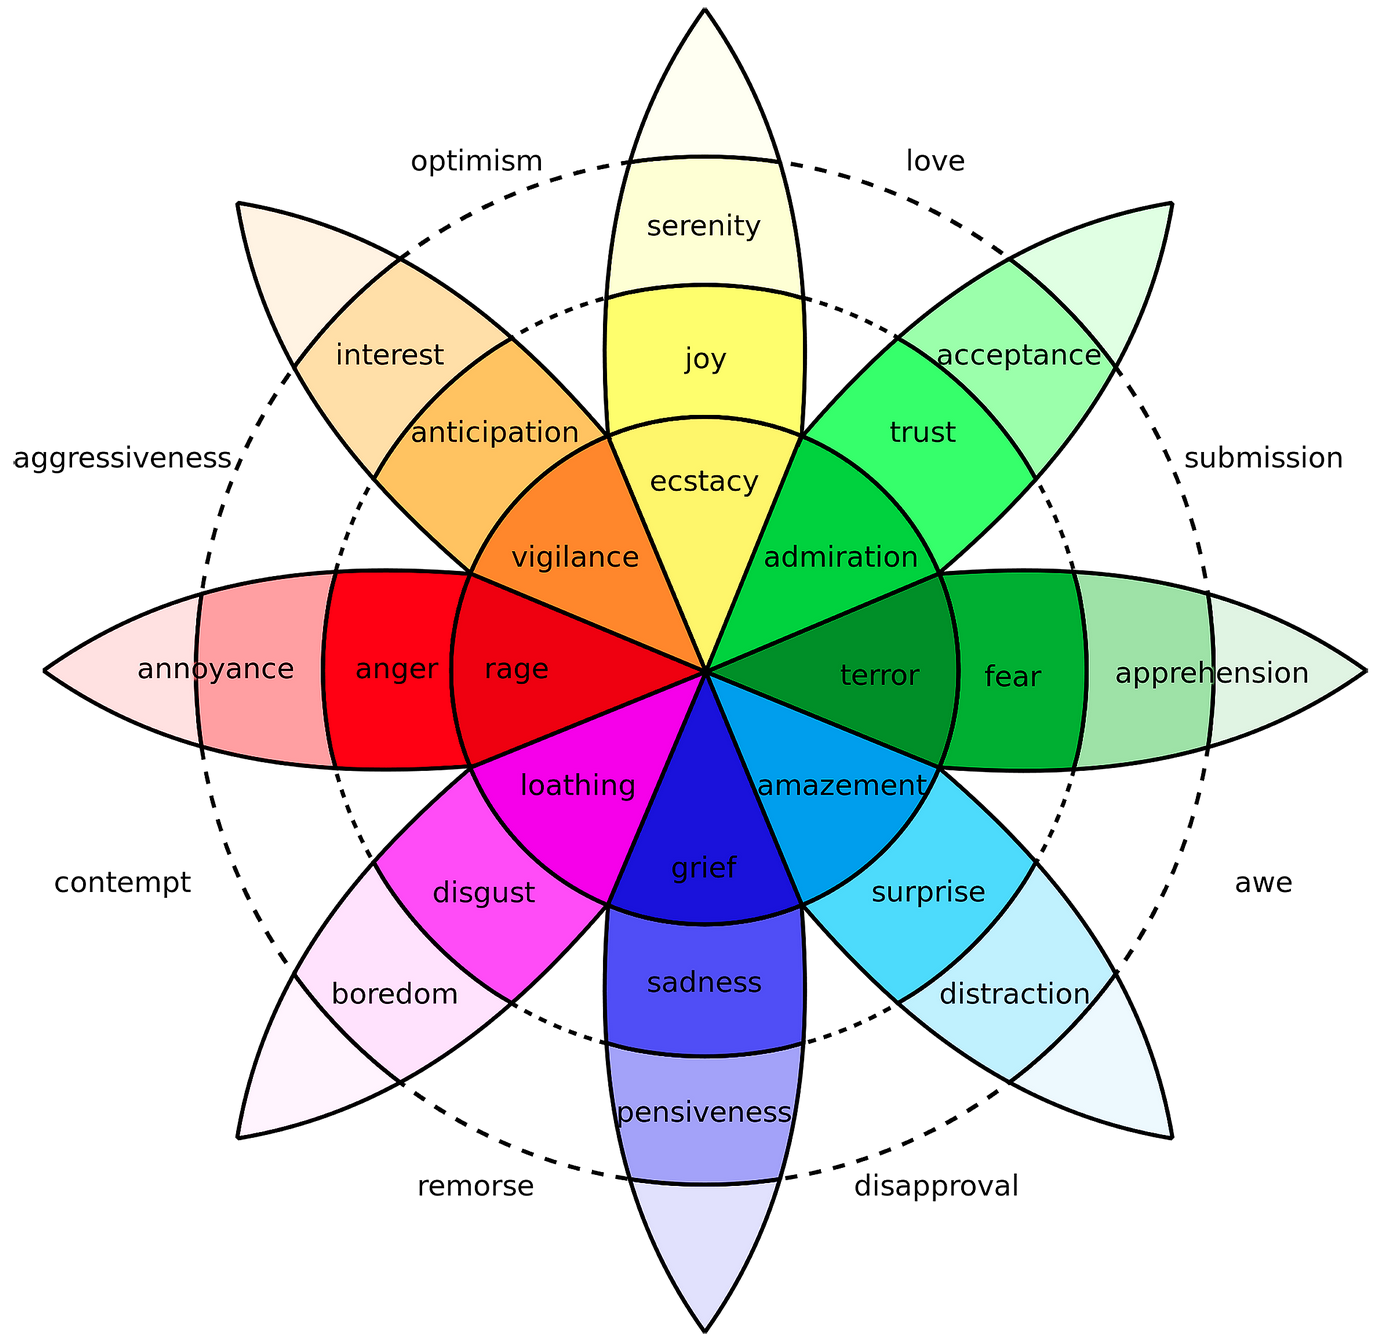
\includegraphics[width=12cm]{/Volumes/Mac OS Drive/Thesis/Source Code/Reporting/nwm_Report/images/Plutchik_wheel_of_emotion.png}
\caption{\label{fig:wheel-of-emotion}Plutchik's \emph{Wheel of Emotion} - eight axes define eight basic emotions, neighbouring pairs of which are used to derive eight \emph{compound emotions}, given between each basic pair on the outskirts of the wheel. The colour-intensity of each axis signifies the intensity of that basic emotion. Darker colours, moving towards the centre of the wheel, represent larger magnitudes of emotion.}
\end{figure}

The second of the two fundamental ideas behind this model is that the dictionary used should not be a limiting factor for the analysis of sentiment within text. What this translates into, practically speaking, is an extremely large dictionary of emotions being desired. This was achieved through applying a separate methodology, namely \href{https://en.wikipedia.org/wiki/Crowdsourcing}{\emph{crowd-sourcing$^{\dag{}}$}}, (comparable to \emph{crowd-funding}) a term springing mainly from online collaborations, whereby many people each make a small contribution to a large project. In this case, people were paid a small amount for each pre-defined batch of words that they manually assigned sentiment scores to.


\subsubsection{Sentiment140}
\label{sec-1-4-2}

This SAM is based on a lexicon that originates from the creators of EmoLex\footnote{There are \href{http://saifmohammad.com/WebPages/lexicons.html}{numerous additional dictionaries defined by EmoLex creator Saif Mohammed$^{\dag{}}$.}}, but differs to it by the method of its creation, in that an \textbf{automated} process was used (detailed below). Such a process has the benefit of being able to assess and learn from many more words than were used for the manually assigned scores of EmoLex. The algorithm is explained in detail within the literature \cite{MohammadKZ2013}; here we provide an explanation only of the essential points.

From a corpus of tweets that each contained an emoji, all possible unigram (one-word) and bigram (two-word) combinations were made from the words contained in that tweet, any non-intelligible cases being subsequently removed via a customised filter. Each unigram and bigram was then assigned a value of $-5$, $0$ or $+5$ depending on the related emoji's predefined score. In total 1.6 million data points were created, and assigned value using this pre-definined dictionary of emojis. The scores assigned to the uni- and bigrams were then used to construct a new dictionary, which can itself be used to evaluate new tweets. The scores of all contained uni- and bigrams within a single tweet are summed to provide the final result.

That the output from the Sentiment140 model can clearly be in the form of large numbers (given each dictionary entry corresponds to either $-5$, $0$ or $+5$) is irrelevant for this study, as all data was later normalised to a smaller range - see Section \texttt{rescaling-sent} for more details.


\subsubsection{SentiStrength}
\label{sec-1-4-3}

This SAM was selected in order to add further diversity to the methodologies used within the five models. The SentiStrength method \cite{Thelwall:2010:SSS:1890706.1890713}, \href{http://sentistrength.wlv.ac.uk/}{available in fifteen languages$^{\dag{}}$}, presents a novel method of analysing sentiment stemming from concepts within the field of psychology - with the notion that humans experience more than one emotion at the same time, with the larger emotions overwhelming the smaller emotions. Expressed differently, each time a person experiences a feeling towards a given event or object, it can be measured on more than one axis, in fact the model outlines three distinct axes. Given an event, defined as anything that may evoke an emotion, three levels of emotion are mapped to these three independent axes, where:

\begin{center}
   \begin{minipage}[c]{65mm} 
   \raggedright % so the minipage's text is left justified
      \textbf{Axis 1:} describes positivity \newline
      \textbf{Axis 2:} describes negativity \newline
      \textbf{Axis 3:} describes neutrality \newline
  \end{minipage}
\end{center}

\vspace{-3mm}

This approach decomposes human emotion, using parameterization to describe something we often experience, and would indeed describe, as one single emotion or feeling. For the purposes of this study, a binary response was chosen, leaving out neutrality. This is because a sense of neutrality can be inferred from the magnitude of the first two axes. If low scores are obtained from both positive and negative feelings regarding an event, then the neutrality score must be relatively high. The results from the binary positive-negative scale were obtained and later combined in the modelling preparation steps outlined in Section \texttt{rescaling-sent}.


\subsubsection{VADER and VADER AFinn \label{vader}}
\label{sec-1-4-4}

\textbf{V}alence \textbf{A}ware \textbf{D}ictionary for s\textbf{E}ntiment \textbf{R}easoning (VADER) - is a parsimonious rule-based model for sentiment analysis of social media \cite{hutto2014vader}. The creators constructed a dictionary targeted towards micro-blogging content e.g. Twitter, via a combination of both quantitative and qualitative methods. At the heart of the algorithm are five simple rules that describe both grammatical and syntactical conventions that are honed to detect markers of sentiment (or \emph{Valence} in VADER terminology) with text. The authors claim that their model not only improves many well-established benchmarks that use more complicated methods, but also outperforms individual human raters. A useful facet of being derived solely using parsimonious techniques is that the model can be generalised quite well into other domains beyond Twitter.

VADER not only includes emojis, but also incorporates common slang terms (e.g. "nah" and "meh"), but also acronyms and initialisms, such as the widely used terms "LOL" and "WTF". Like many other creators of sentiment analysis dictionaries, the authors made use of \href{https://www.mturk.com/mturk/welcome}{Amazon Mechanical Turk$^{\dag{}}$}\footnote{A system whereby \emph{employers} create tasks to be completed, (usually repetitive and not requiring any introduction) that \emph{employees} can slowly work through at any given time. It means humans perform the work and is an extension of crowd sourcing, mentioned in section \ref{emolex}.}, meaning each of their words was \textbf{manually} assigned a value by a human. The authors also created some extra steps to this process (detailed in the above referenced literature) to ensure that the evaluation of all tweets was performed to the highest standard, to produce what they term a \emph{gold-standard} lexicon. This is a crucial point, considering the model itself uses only a small number of rules to classify tweets as positive or negative.

\vspace{5mm} \noindent
VADER AFinn, built upon the VADER lexicon (the AFinn suffix derived from the author's name) defines yet another lexicon, which includes higher amounts of slang and even \href{https://simple.wiktionary.org/wiki/Category:Vulgar}{\emph{vulgar slang$^{\dag{}}$}} - words that not many lexicons include, but are commonly seen on micro-blogging websites. In the related literature, \cite{NielsenF2011New}, the author shows several examples where the inclusion of such words does indeed more accurately reflect the true sentiment of the text. Syntactical analysis is also performed just as in VADER, where e.g. the words "but" is used in the quantification step as a contrastive conjunction. This means that "but" makes a contrast where the text that follows it reflects a stronger sentiment than the text preceding it. The tweet text before is reduced in intensity and the text following is increased in intensity to take this into account.


\subsubsection{Example analyses}
\label{sec-1-4-5}

All tweets taken and cleaned from Twitter Mining saved in text files with one tweet per line read through each sentiment model, outputs returned in one table. Table \ref{tab:tweet-examples} contains scores provided by the different SAMs for several sample tweets. Without describing in great deal how the results differ, it is clear that the described features of each model do have an impact when analysing informal text, as found within the Twitter data. Worth noting are (1) the binary output from the SentiStrength model, the first results representing how \emph{negative} the tweet is and the second how \emph{positive}, and (2) the zero value for VADER in Example 3. The two values of both halves of the sentence in \texttt{Example 3} balance out to create an overall zero outcome, which is not observed in the other models. The results for the same tweet, being relatively negative for all other models, reflects the property in the model described in Section \ref{vader}, using conjuntions such as "but" to accordingly weight the main and subordinate clauses being connected. 

\begin{table}[htb]
\centering
\begin{tabular}{clccccc}
\textbf{ID} & \textbf{Tweet text} & \textbf{EmoLex} & \textbf{Sentiment140} & \textbf{SentiStrength} & \textbf{VADER} & \textbf{V. AFinn}\\
 &  &  &  &  &  & \\
\hline
 &  &  &  &  &  & \\
1 & I love you :-) LOL & $+$ 0.7 & $+$ 0.6 & ($-$ 1, $+$ 4) & $+$ 0.8 & $+$ 1.0\\
2 & I hate you :-( & $-$ 0.9 & $-$ 0.9 & ($-$ 5, $+$ 1) & $-$ 0.8 & $-$ 1.0\\
3 & I like cats, but hate dogs & $-$ 0.3 & $-$ 0.1 & ($-$ 4, $+$ 3) & 0 & $-$ 0.5\\
 &  &  &  &  &  & \\
\end{tabular}\caption{\label{tab:tweet-examples}Three example tweets with sentiment scores from each model.}

\end{table}


\subsection{Applications in finance}
\label{sec-1-5}

Here we give three examples of related works, which display how sentiment analysis can be applied within a financial setting, and how it indeed was at different points over the past decade.


\subsubsection{In 2006}
\label{sec-1-5-1}

Baker and Wurgler, \cite{JOFI:JOFI885}, created and implemented a sentiment driven model to investigate cross-sections of returns. Up until that point in time, classical financial theory was used to explain how the diversification methods among rational investors leads to an equilibrium in the market, which precisely portrays all rationally discounted cash flows. This general statement is supported by the Efficient Market Hypothesis (EMH), defined by Fama \cite{malkiel1970efficient} as follows: "\emph{prices fully and instantaneously reflect all publicly available information}"\footnote{Alternatively formulated from the perspective of arbitrage by Jensen \cite{jensen1978some}: "A market is efficient with respect to an information set, if it is impossible to make economic profits by trading on the basis of this information".}. The work carried out by Baker and Wurgler involved defining three \emph{proxies} to investor sentiment (there was no social media data readily available at the time), which were: the book-to-market ratio, external financing and sales growth. The authors recognised that these were not direct indicators of sentiment, hence naming them proxies, and so took the first principal component of the data set as the final variable.
They were able to make two statements from their results regarding the reurns of certain categories of stocks\footnote{Small stocks, young stocks, high volatility stocks, unprofitable stocks, non-dividend-paying stocks, extreme growth stocks, and distressed stocks.}:

\begin{enumerate}
\item when beginning-of-period proxies for sentiment are low, subsequent returns are relatively high, but
\item when sentiment is high, relatively low subsequent returns may be expected.
\end{enumerate}


\subsubsection{In 2010}
\label{sec-1-5-2}

Bollen \emph{et al.} \cite{DBLP:journals/corr/abs-1010-3003} show how Twitter sentiment can be used to predict stock markets movements using sentiment results from two different SAMs (\href{http://mpqa.cs.pitt.edu/opinionfinder/}{OpinionFinder$^{\dag{}}$} and Google-Profile of Mood States (GPOMS)\footnote{This is a modified version of a \href{http://www.brianmac.co.uk/poms.htm}{well-known psycological test$^{\dag{}}$}, which was adapted by the authors for use with Google data.}). The GPOMS model is similar to the EmoLex model described in Section \ref{emolex}, defining various scales of emotion. Using one of these elements along with historical market data within a self-organising fuzzy neural network model, the authors were able to make predictions regarding market movement with accuracies greater than 80 \%. The work was influenced by ideas stemming from behavioural finance, the authors being able to gain Kahneman's input (see Section \ref{sent-defn}) regarding their model and utilising notions from his Prospect Theory.


\subsubsection{In 2012 and beyond}
\label{sec-1-5-3}

The last example is that of major ongoing project \href{https://www.marketpsych.com/guide/}{MarketPsych$^{\dag{}}$}, an index of sentiment compiled by Thomson Reuters over a vast number of industries. Many sources of data are used, but are able to be placed into three categories: high-frequency data in the form of social media messages from 1998 to present, medium frequency data obtained through the trawling (web-scraping) of countless internet news sites and live, low frequency data obtained directly from Retures itself. The algorithms that follow are very similar to those employed in this study, with all the information boiling down to numerical indicators. These are what form the Thomson Reuters MarketPsych Indices (TRMI), which had modest beginnings, only covering several general asset classes (such as agriculture and energy), but now includes many thousands of indicators going as far as focusing on specific companies.
One great area of success shown by TRMI has been the recognition and \href{http://thomsonreuters.com/en/articles/2015/understanding-bubbles.html}{prediction of market bubbles$^{\dag{}}$}. Arguing that bubbles are no longer only sparse events, they instead - with the rapidly growing international connectivity and corresponding currents of money within financial markets - additionally describe short-lived \emph{specultive mania}, which the real-time analysis of sentiment data allows investors to track.


\bibliographystyle{plain}
\bibliography{references}
% Emacs 24.5.1 (Org mode 8.2.10)
\end{document}